\section{Combined Analysis}\label{sec:formal}

In this section, we formally define the combined analysis with sealed symbolic
execution.  We extend the formalization of abstract interpretation and analysis
sensitivity proposed by \citet{sens-toplas}.


\subsection{Concrete Semantics}

We define a program $\prog$ as a state transition system $(\stset, \trans,
\istset)$.  A program starts with an initial state in $\istset$ and the
transition relation $\trans \subseteq \stset \times \stset$ describes how states
are transformed to other states.  A \textit{collecting semantics} $\sem{\prog} =
\{ \st \in \stset \mid \ist \in \istset \wedge \ist \trans^* \st \}$ consists of
reachable states from initial states of the program $\prog$.  We could calculate
it using the \textit{transfer function} $\transfer: \dom \rightarrow \dom$ as
follows:
\[
  \sem{\prog} = \underset{n \rightarrow \infty}{\lim}{\transfer^n(\ielem)}\\
  \qquad
  \transfer(\elem) = \elem \join \step(\elem)\\
\]
The \textit{concrete domain} $\dom = \powerset{\stset}$ is a complete lattice
with $\cup$, $\cap$, and $\subseteq$ as its join($\join$), meet($\meet$), and
partial order($\order$) operators.  The element $\ielem$ denotes the initial
states $\istset$.  The \textit{one-step execution} $\step: \dom \rightarrow
\dom$ transforms states using the transition relation $\trans$: $\step(\elem) =
\{ \st' \mid \st \in \elem \wedge \st \trans \st' \}$.

\begin{figure}[H]
  \[
    \begin{array}{l}
      \enspace \labdot{0} \; \varx = \;? \; ;  \; \labdot{1}\\
      \enspace \kwif \; (\; \varx \geq 0 \;) \; \labdot{2} \; \varx = \varx ;\\
      \enspace \kwelse \; \labdot{3} \; \varx = -\varx ;  \; \labdot{4}\\
    \end{array}
  \]
  \vspace*{-1em}
  \caption{Conditional branch}
  \label{fig:running-example}
\end{figure}

For example, the code in Figure~\ref{fig:running-example} is a simple program
that applies the mathematical absolute value function to the variable $\varx$.
The question mark $?$ denotes the user input that returns an integer.  States
are pairs of labels and integers $\varx$: $\stset = \labset \times \mathbb{N}$.
The initial states are $\istset = \{ (\lab_0, 0) \}$ which means the program
starts with the varible $\varx$ that stores 0 at $\lab_0$.  If the user input is
$-42$, the program is executed with the following trace:
\[
  (\lab_0, 0) \trans (\lab_1, -42) \trans (\lab_3, -42) \trans (\lab_4, 42)
\]

\subsection{Abstract Interpretation}
The abstract interpretation~\cite{abs-interp-1977, abs-interp-1992}
over-approximates the transfer $\transfer$ to the \textit{abstract transfer
function} $\abstransfer: \absdom \rightarrow \absdom$ to get the
\textit{abstract semantics} $\abssem{\prog}$ in finite iterations as follows:
\[
    \abssem{\prog} = \underset{n \rightarrow
    \infty}{\lim}{(\abstransfer)^n(\iabselem)}\\
\]
We define a \textit{state abstraction} $\dom \galois{\alpha}{\gamma} \absdom$ as
a Galois connection between the concrete domain $\dom$ and an abstract domain
$\absdom$ with a \textit{concretization function} $\gamma$ and an
\textit{abstraction function} $\alpha$.  The initial abstract state $\iabselem
\in \absdom$ represents an abstraction of the initial state set; $\ielem
\subseteq \gamma(\iabselem)$.  The abstract transfer function $\abstransfer:
\absdom \rightarrow \absdom$ is defined as $\abstransfer(\abselem) = \abselem
\join \absstep(\abselem)$ with an \textit{abstract one-step execution}
$\absstep: \absdom \rightarrow \absdom$.  For the sound state abstraction, the
join operator and the abstract one-step execution should satisfy the following
conditions:
\begin{itemize}
  \item $\forall \abselem_0, \abselem_1 \in \absdom. \; \gamma(\abselem_0) \cup
    \gamma(\abselem_1) \subseteq \gamma(\abselem_0 \join \abselem_1)$
  \item $\forall \abselem \in \absdom. \; \absstep \circ \gamma(\abselem) \subseteq
    \gamma \circ \absstep(\abselem)$
\end{itemize}

A simple example abstract domain is $\absdom_\pm = \powerset{\{ -, +, 0 \}}$ with
set operators as domain operators; $-$ denotes negative integers, $+$ positive
integers, and $0$ zero.  If we use it for the code in
Figure~\ref{fig:running-example}, the analysis result becomes $\{ -, +, 0 \}$
because $\varx$ can have any integers at $\lab_1$.


\subsection{Analysis Sensitivity}

Abstract interpretation is often defined with \textit{analysis sensitivity} to
increase the precision of static analysis.  A sensitive abstract domain
$\sabsdom: \viewset \rightarrow \absdom$ is defined with a \textit{view
abstraction} $\viewmap: \viewset \rightarrow \dom$ that provides multiple points
of views for reachable states during static analysis.  It maps a finite number
of views $\viewset$ to sets of states $\dom$. Each view $\view \in \viewset$
represents a set of states $\viewmap(\view)$.
A \textit{sensitive state abstraction} $\dom
\galois{\alpha_\viewmap}{\gamma_\viewmap} \sabsdom$ is a Galois connection between
the concrete domain $\dom$ and the sensitive abstract domain $\sabsdom$ with the
following concretization function:
\[
  \gamma_\viewmap(\sabselem) = \{ \st \in \stset \mid \forall \view \in \viewset.
  \; \st \in \viewmap(\view) \Rightarrow \st \in \gamma \circ \sabselem(\view) \}
\]

With analysis sensitivities, the abstract one-step execution $\sabsstep:
\sabsdom \rightarrow \sabsdom$ is defined as follows:
\[
  \sabsstep(\sabselem) = \lambda \view \in \viewset. \; \underset{\view' \in
  \viewset}{\bigjoin}{\viewtrans{\view'}{\view} \circ \sabselem(\view')}
\]
where $\viewtrans{\view'}{\view}: \absdom \rightarrow \absdom$ is the abstract
semantics of a \textit{view transition} from a view $\view'$ to another view
$\view$.  It should satsify the following condition for the soundness of the
analysis:
\[
  \forall \abselem \in \absdom. \; \step(\gamma(\abselem) \cap \viewmap(\view'))
  \cap \viewmap(\view) \subseteq \gamma \circ
  \viewtrans{\view'}{\view}(\abselem)
\]

One of the most widely-used analysis sensitivity is \textit{flow sensitivity}
defined with the flow-sensitive view abstraction $\fsviewmap: \labset
\rightarrow \dom$ where
\[
  \forall \lab\in\labset. \; \fsviewmap(\lab) = \{ \st \mid \st = (\lab, \_) \}
\]
If we apply the flow sensitivity for the above example, the analysis result
becomes as follows:
\[
  \begin{array}{|c||c|c|c|c|c|}\hline
    \labset & \lab_0 & \lab_1 & \lab_2 & \lab_3 & \lab_4\\\hline
    \absdom_\pm & 0 & -, +, 0 & +, 0 & - & +, 0\\\hline
  \end{array}
\]


\subsection{Sealed Symbolic Execution}

To handle abstract values in concrete semantics, we define \textit{sealed
symbolic execution} by extending the transition relation $\trans$ as a symbolic
transition relation $\symbtrans$ on symbolic states.  First, we extends the
concrete states $\stset$ to symbolic states with \textit{sealed symbolic values}
$\symbset$.  A symbolic transition relation $\symbtrans \subseteq \symbstset
\times (\symbstset \uplus \{ \excst \})$ is exactly the same with the original
transition relation $\trans$ except when the relation requires the exact value
of sealed symbolic values.  In this case, the symbolic state has the relation a
special exception state $\excst$ to represent that it is impossible to interpret
in a concrete way.  Thus, a symbolic state \textit{always} has a symbolic
transition relation with a single symbolic state, and the sealed symbolic
execution is linear until being terminated or reaching the exception state
$\excst$.

The main difference of sealed symbolic execution with the traditional symbolic
execution~\cite{symbolic} is that it only supports sealed symbolic values
instead of symbolic expressions and path constraints.  For example, the
following trace represents the traditional symbolic execution of the running
example in Figure~\ref{fig:running-example}:
\[
  \begin{array}{r@{~}c@{~}l}
    &&(\lab_2, \symb)[\symb \geq 0] \trans (\lab_4, \symb)[\symb \geq 0]
    \vspace*{-0.5em}\\
    &\rutrans&
    \vspace*{-0.5em}\\
    (\lab_0, 0)[] \trans (\lab_1, \symb)[]&&
    \vspace*{-0.5em}\\
    &\rdtrans&
    \vspace*{-0.5em}\\
    &&(\lab_3, \symb)[\symb < 0] \trans (\lab_4, -\symb)[\symb < 0]\\
  \end{array}
\]
It first assigns a symbolic value $\symb$ to the variable $\varx$ at $\lab_1$.
For the conditional branch, it is forked by creating two symbolic states with
different path conditions $\symb \geq 0$ and $\symb < 0$ for true and false
branches, respectively.  After executing statements $\varx = \varx$ and $\varx =
-\varx$, the variable $\varx$ stores symblic expressions $\symb$ and $-\symb$ at
$\lab_4$.  However, the sealed symbolic execution stops at $\lab_1$ as follows:
\[
  (\lab_0, 0) \; \symbtrans \; (\lab_1, \symb) \; \symbtrans \; \excst
\]
because the branch requires the actual value of the symbolic value $\symb$.

To freely convert a pair of view and an abstract state to its corresponding
symbolic state and vice versa, we define two domain converters $\symbstset
\galois{\saconverter}{\asconverter} (\viewset \times \absdom)$.  In the
converter $\asconverter$ from abstract states to symbolic states, if an abstract
value $\absval$ represents a singleton value, the function transforms the
abstract value to the corresponding concrete value.  Otherwise, it converts the
abstract value as a symbolic value in a result symbolic state.  Two converters
convert given elements wihtout loss of information:
\[
  \saconverter \circ \asconverter = \asconverter \circ \saconverter = \identity
\]
where $\identity$ denotes the identity function.


\subsection{Combined Analysis}

\begin{figure}[t]
  \centering
  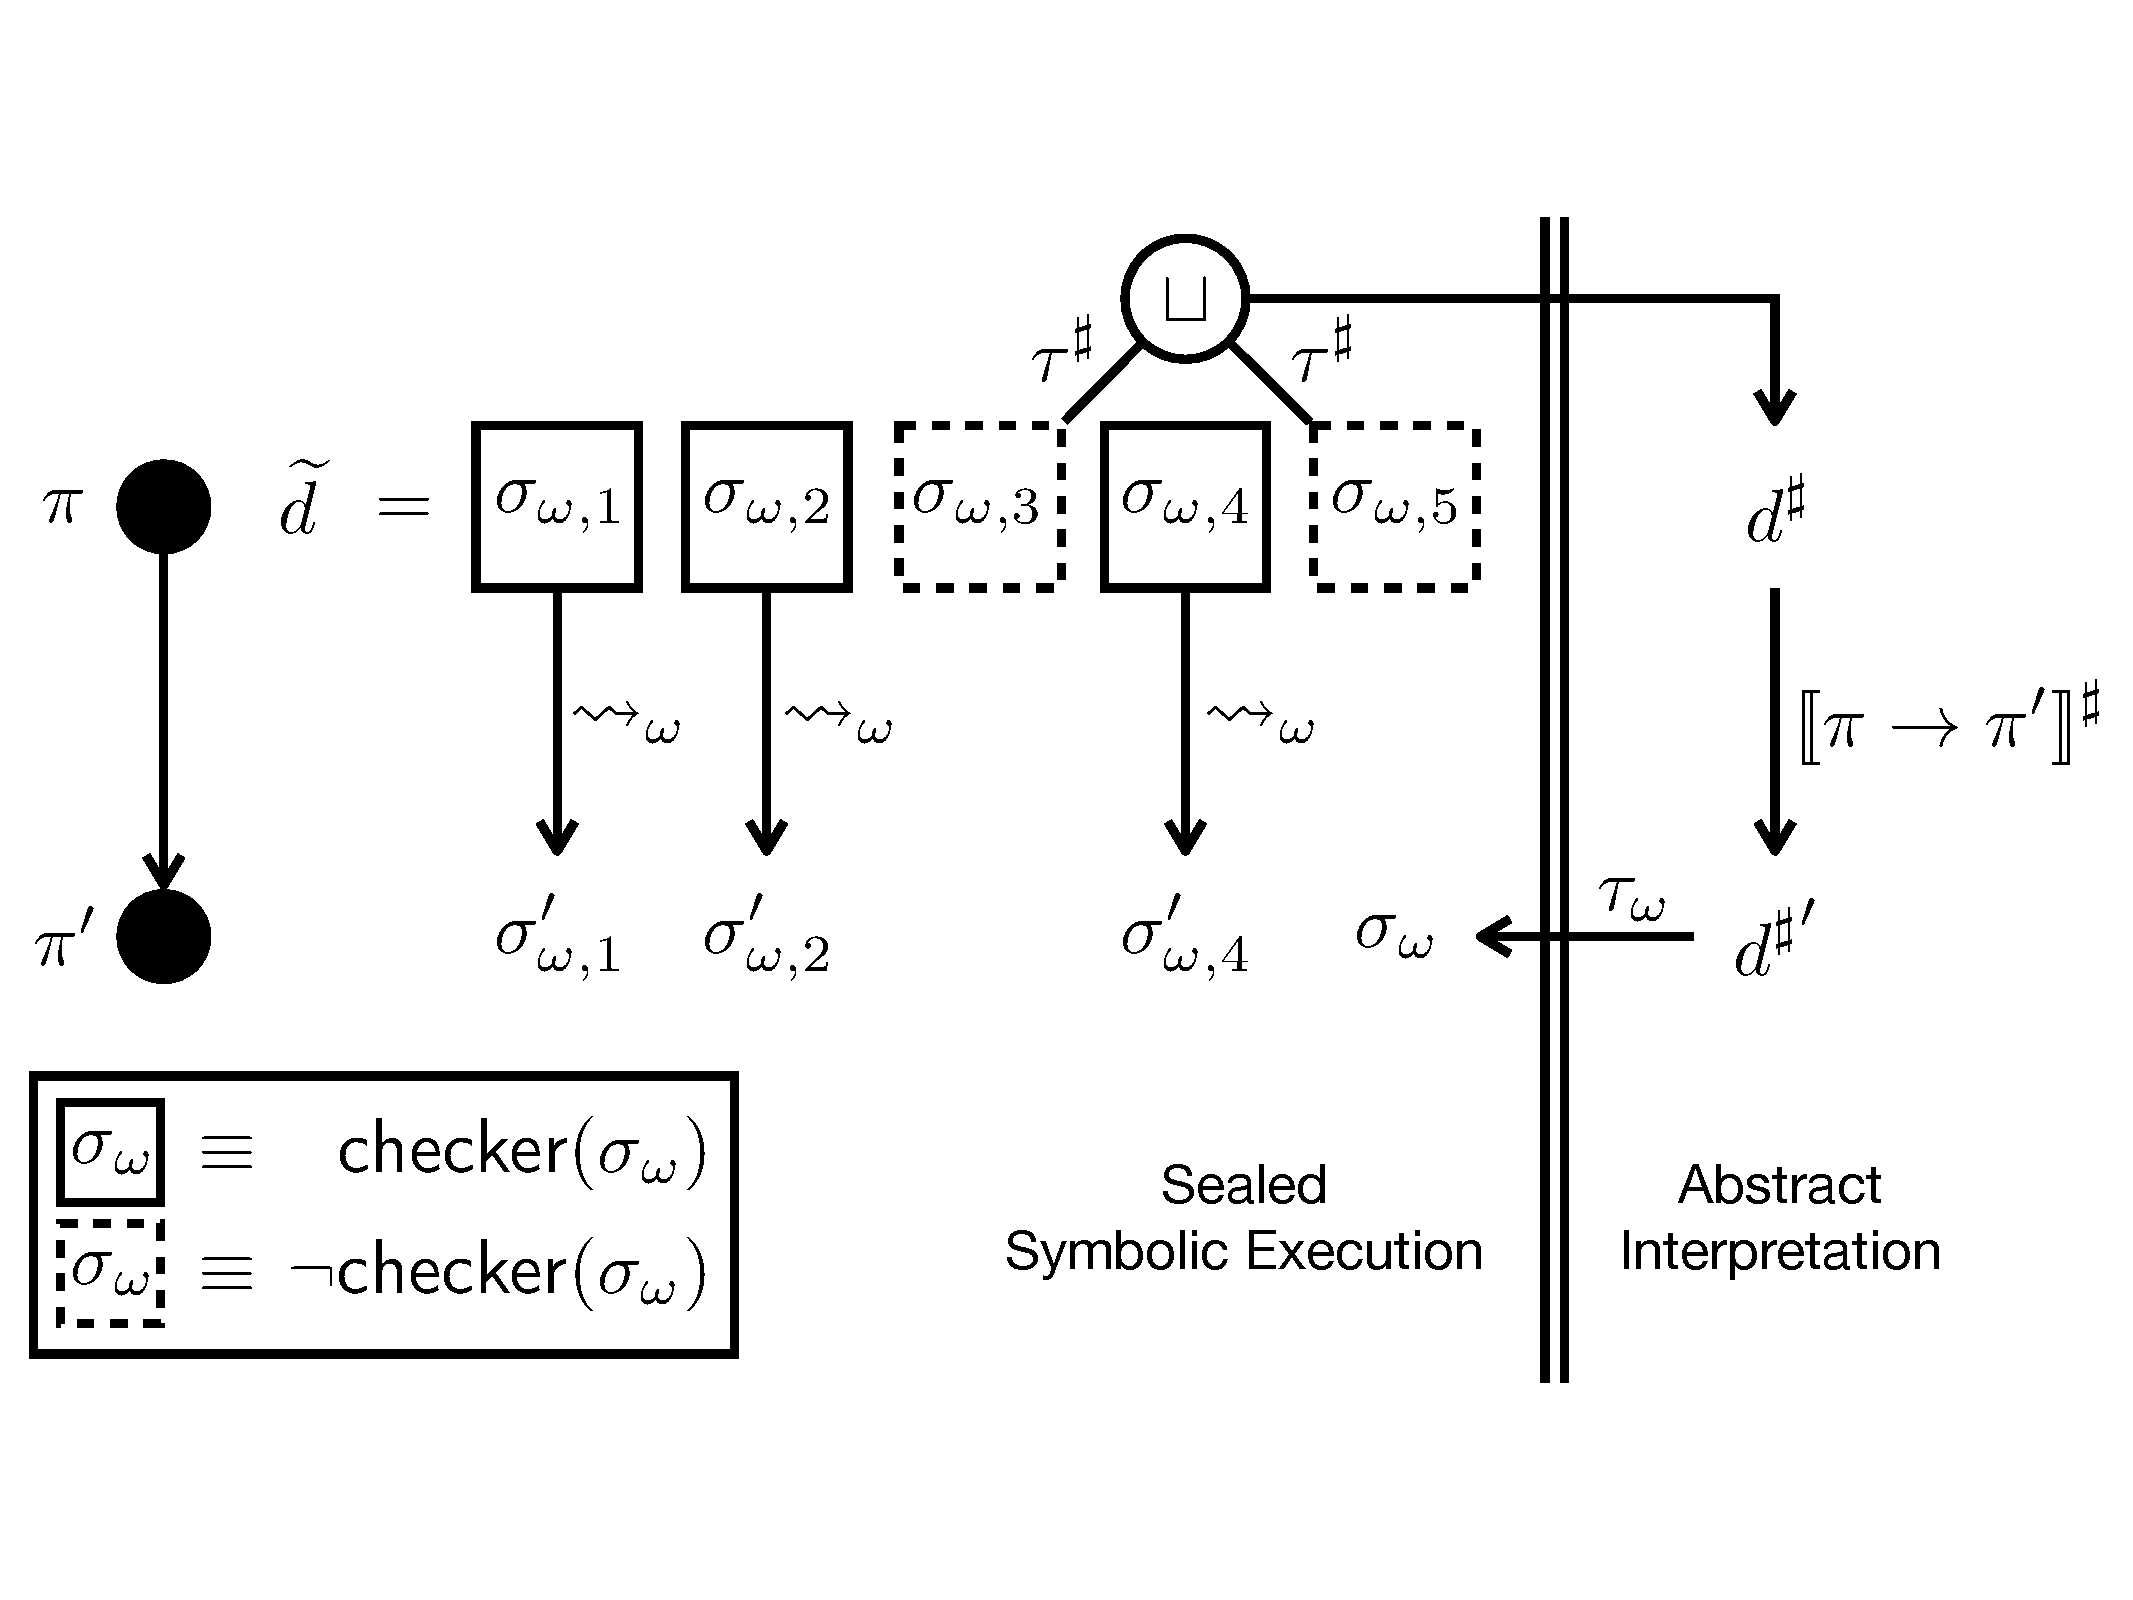
\includegraphics[width=\linewidth]{img/combined-analysis}
  \vspace*{-2em}
  \caption{The diagram for the extended view transition in the combined analysis.}
  \vspace*{-1em}
  \label{fig:combined-analysis}
\end{figure}

We define the \textit{combined analysis} of the abstract interpretation and the
sealed symbolic execution.  In the combined analysis, we use the powerset of
symbolic states as the domain $\combdom = \powerset{\symbstset}$, and extend the
view transition as follows:
\[
  \begin{array}{l}
    \combviewtrans{\view}{\view'}(\combelem) =\\
    \qquad \{
      \symbst' \mid \symbst \in S \wedge
      \symbst \symbtrans \symbst' \wedge
      \saconverter(\symbst') = (\view', \_)
    \}\\
    \qquad \cup \left\{
    \begin{array}{ll}
      \{ \asconverter \circ \viewtrans{\view}{\view'}(\bigjoin D) \}
      & \text{if} \; D \neq \varnothing\\
      \varnothing & \text{otherwise}\\
    \end{array}
    \right.
  \end{array}
\]
where $S = \combelem\mid_{\checker}$ and $D =
\dot{\saconverter}(\combelem\mid_{\neg\checker})$.  The dot notation $\dot{f}$
denotes the element-wise extended function of a function $f$.  The combined
analysis performs one-step symbolic transition for each symbolic state that
passes the filter $\checker$. On the other hand, it converts remaining symbolic
states to the corresponding abstract states, merges them into a single abstract
state, and performs the abstract one-step execution for the abstract state.

For example, Figure~\ref{fig:combined-analysis} depicts the
diagram of the view transition from $\view$ to $\view'$ in the combined
analysis.  The element $\combelem$ in $\view$ consists of five symbolic states
from $\nsymbst{1}$ to $\nsymbst{5}$.  The solid box denotes that the corresponding
symbolic state passes the filter $\checker$ and the dotted box denotes that it
does not.  For each symbolic state that passes the filter ($\nsymbst{1}$,
$\nsymbst{2}$, and $\nsymbst{4}$), it applies the symbolic transition $\symbtrans$.
For failed symbolic states ($\nsymbst{3}$ and $\nsymbst{5}$), it applies the
converter $\saconverter$ to convert each of them to the corresponding abstract
state and merges results using the join operator ($\join$).  Then, it utilizes
the abstract semantics via the original view transition
$\viewtrans{\view}{\view'}$ and the converter $\asconverter$ to convert the
result to the corresponding symbolic state.

We could configure when the sealed symbolic execution or the abstract
interpretation is performed based on the definition of the $\checker$ function
and its negation $\neg\checker$.  For example, we could define the $\checker$
that passes only function entry, call, and exit points to perform conversions in
a function level.  However, for the soundness and the termination of the
combined analysis, it should satisfy the following condition:
\begin{theorem}
  The combined analysis has sound analysis result and terminates in a finite
  time if its abstract semantics is sound and $\checker$ satisfies the following
  condition:
  \[
    \checker(\symbst) \Rightarrow \symbst \symbtrans^k \excst \wedge
    1 < k \leq N
  \]
  where $N$ is a pre-defined maximum length of the sealed symbolic execution.
\end{theorem}
\inred{We prove that any combined analysis defined with the extended view
transition satisfying the above condition always has sound analysis result and
terminates in a finite time. Because of the page limitation, we omit the
proof in this paper and include it in a companion report.}
